\section*{Exponential Decay}
\textcolor{red}{TODO: Radioactive decay, half life, motivation of rational exponents}

We have already seen an example of exponential growth.
Now we are going to examine the exponential decay.

Many atoms are unstable in the sense that they can decay into two atoms of with a smaller core.
This phenomenon is called ``radioactive decay''.
An important example is the carbon atom, or more precisely, the \ce{^{14}C} isotope of carbon.
It is know to have a \textbf{half-live} of 5730 years, that is
\begin{center}
	every \ce{^{14}C} atom has a probability of 50\% to decay with the next 5730 years.
\end{center}
Put differently, for any given an amount $a$ of \ce{^{14}C} atoms, we expect that after 5730 years, half of them will have decayed, so that we are left with $\frac{a}{2}$ atoms.
After another 5730 years we will be left with half of $\frac{a}{2}$, i.e. with $\frac{a}{4}$.
We arrive at the following table.
\begin{figure}[ht]
	\centering
	\begin{tikzpicture}
		\matrix[matrix of math nodes,draw, column sep=1em,row sep=.5mm] (mx) {
			\textrm{year} & 0 & 5730 & 11460 & 17190 & 22920 & 28650 & 34380 \\
			\textrm{atoms} & \phantom{\frac{a}{1}}a\phantom{\frac{a}{1}} & \frac{a}{2} & \frac{a}{2^2} & \frac{a}{2^3} & \frac{a}{2^4} & \frac{a}{2^5} & \frac{a}{2^6} \\
		};
		\path[->,shorten >=2pt]
		\foreach \from/\to in {2/3,3/4,4/5,5/6,6/7,7/8} {
			([yshift=2mm]mx-1-\from.north) edge[bend left]
			node[above] {$\scriptstyle+5730$} ([yshift=2mm]mx-1-\to.north)
			([yshift=-2.5mm]mx-2-\from.south) edge[bend right]
			node[below] {$\scriptstyle\cdot\frac{1}{2}$} ([yshift=-2.5mm]mx-2-\to.south)
		};
		\foreach \x in {2,...,8}{
			\draw ([xshift=-1em]mx.north west -| mx-1-\x.west) -- ([xshift=-1em]mx.south west -| mx-1-\x.west);
		};
		\draw (mx.west) -- (mx.east);
	\end{tikzpicture}
\end{figure}
\begin{figure}[ht]
	\centering
	\includegraphics[width=0.49\textwidth]{images/decay}\hfill
	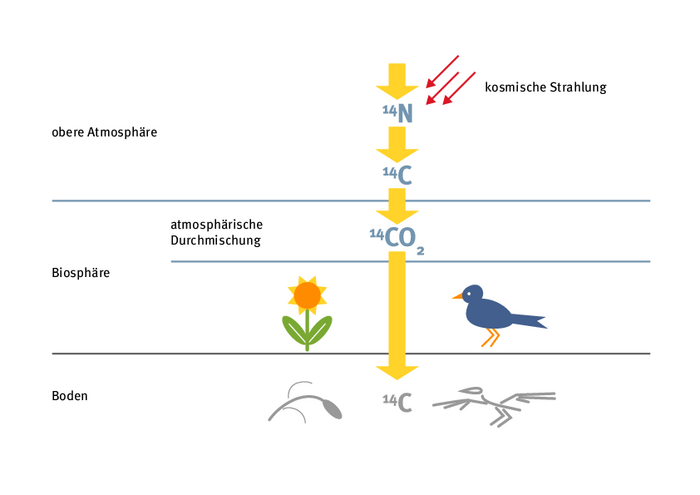
\includegraphics[width=0.49\textwidth]{images/c14_lifecycle}
	\caption{Decay of \ce{^{14}C} with $a=1024$ atoms (left) and the \ce{^{14}C} lifecycle (right).}
	\label{fig:c14}
\end{figure}